\documentclass[graphics]{beamer}
\usepackage{xcolor}
\usepackage{graphicx}
\usepackage{verbatim}
\usepackage{wrapfig}
\usepackage{tabularx}
\usepackage{multirow}
\usepackage{amssymb}
\usepackage{pifont}
\usepackage{tikz}
\def\Checkmark{\tikz\fill[scale=0.2](0,.35) -- (.25,0) -- (1,.7) -- (.25,.15) -- cycle;} 

\useoutertheme{shadow}
%\usecolortheme{orchid}
\usecolortheme{seahorse}
\newcommand{\cmark}{\text{\ding{51}}}
%\newcommand*{\GtrSim}{\smallrel\gtrsim}

% math commands
\newcommand{\be}{\begin{eqnarray}}
\newcommand{\ee}{\end{eqnarray}}
\newcommand{\beq}{\begin{equation}}
\newcommand{\eeq}{\end{equation}}
\def\simless{\mathbin{\lower 3pt\hbox
      {$\rlap{\raise 5pt\hbox{$\char'074$}}\mathchar"7218$}}}
\def\simgreat{\mathbin{\lower 3pt\hbox
      {$\rlap{\raise 5pt\hbox{$\char'076$}}\mathchar"7218$}}} %> or of order

% variables

\def\toonscale{0.45}
\def\mboxy#1{\mbox{\small #1}}

\defbeamertemplate*{title page}{customized}[1][]
{
  \usebeamerfont{title}\inserttitle\par
  \usebeamerfont{subtitle}\usebeamercolor[fg]{subtitle}\insertsubtitle\par
  \bigskip
  \usebeamerfont{author}\insertauthor\par
  \usebeamerfont{institute}\insertinstitute\par
  \usebeamerfont{date}\insertdate\par
  \usebeamercolor[fg]{titlegraphic}\inserttitlegraphic
}
\begin{comment}
\AtBeginSection[]{
  \frame{
    \frametitle{Outline}
    \tableofcontents[currentsection]
  }
}
\end{comment}


\title{\textcolor{red}{Pulsars: Future opportunities for Canada}}
%\subtitle{}
\author[U. Pen]{{
{
}
\textcolor{green}{\small } 
\textcolor{green}{\small Ue-Li Pen}
}
\\[8mm] 
}
\date{May 7, 2019}


\begin{document}

\frame{
\vspace{-0.5in}
\begin{center}  
%\includegraphics[width=4.4in]{Figures/IMG-0438-by-Andre-cropped.jpg}
\end{center}
\begin{picture}(320,250)
%\put(-50,60){
%\includegraphics[width=5.5in]{Figures/GBT_nrao.jpg}}
\end{picture}
\vspace{-4in}
\\
%image credit: NRAO/AUI/NSF
\\
\vspace{1in}
\titlepage
}

%\section*{Introduction}
\section{Introduction}

\begin{comment}
  \subsection{Outline}

  \frame{
    \frametitle{Outline}
    \tableofcontents
  }
\end{comment}

  \frame{
    \frametitle{Overview}
    \begin{itemize}
      \item breakthrough potential:
      \item precision localization of BH GW sources with PTA
      \item discovery of PSR-BH binary
      \item deviations from GR: classical, quantum
    \end{itemize}
  }

  \frame{
    \frametitle{Discovery space}
    \begin{itemize}
      \item milli-second pulsars: limited by computing speed,
        optimized with big telescopes, e.g FAST
      \item slow pulsars: new tree search (K. Smith) opens discovery
        space for transit telescopes
      \item VLBI Scintillometry opens potential for precision
        distances, PTA localization, improved timing, etc
    \end{itemize}
  }

  \frame{
    \frametitle{Optimization}
    \begin{itemize}
      \item slow pulsar search determined by point source sensitivity
      \item CHIME all sky $\sim 10 \mu {\rm K}/\sqrt{\rm yr}$: unprecedented speed
      \item compact array, FFT beamforming, FFT/tree dedispersion,
        FFT/tree folding.
    \end{itemize}
  }

  \frame{
    \frametitle{Coherent radiation}
    \begin{itemize}
      \item most pulsars are coherent point sources 
      \item form interference pattern through ISM/companion lensing
      \item probe plasma green's function
      \item initial tests indicate 50 picoarcsecond astrometry
      \item slow pulsar-BH binary well suited for lensing
        interferometry! (Yang+Pen 2015)
    \end{itemize}
  }


  \frame{
    \frametitle{ISM lenses}
    \begin{itemize}
        \item natural coherent 1-D single screens in the ISM
        \item origin starting to be sorted out: refractive reconnection sheets
        \item paradigm shift from turbulent, volume filling
          diffraction
        \item deployable for precision picroarcsecond interferometry
    \end{itemize}
%\vspace{-0.1in}\hspace{.3in}
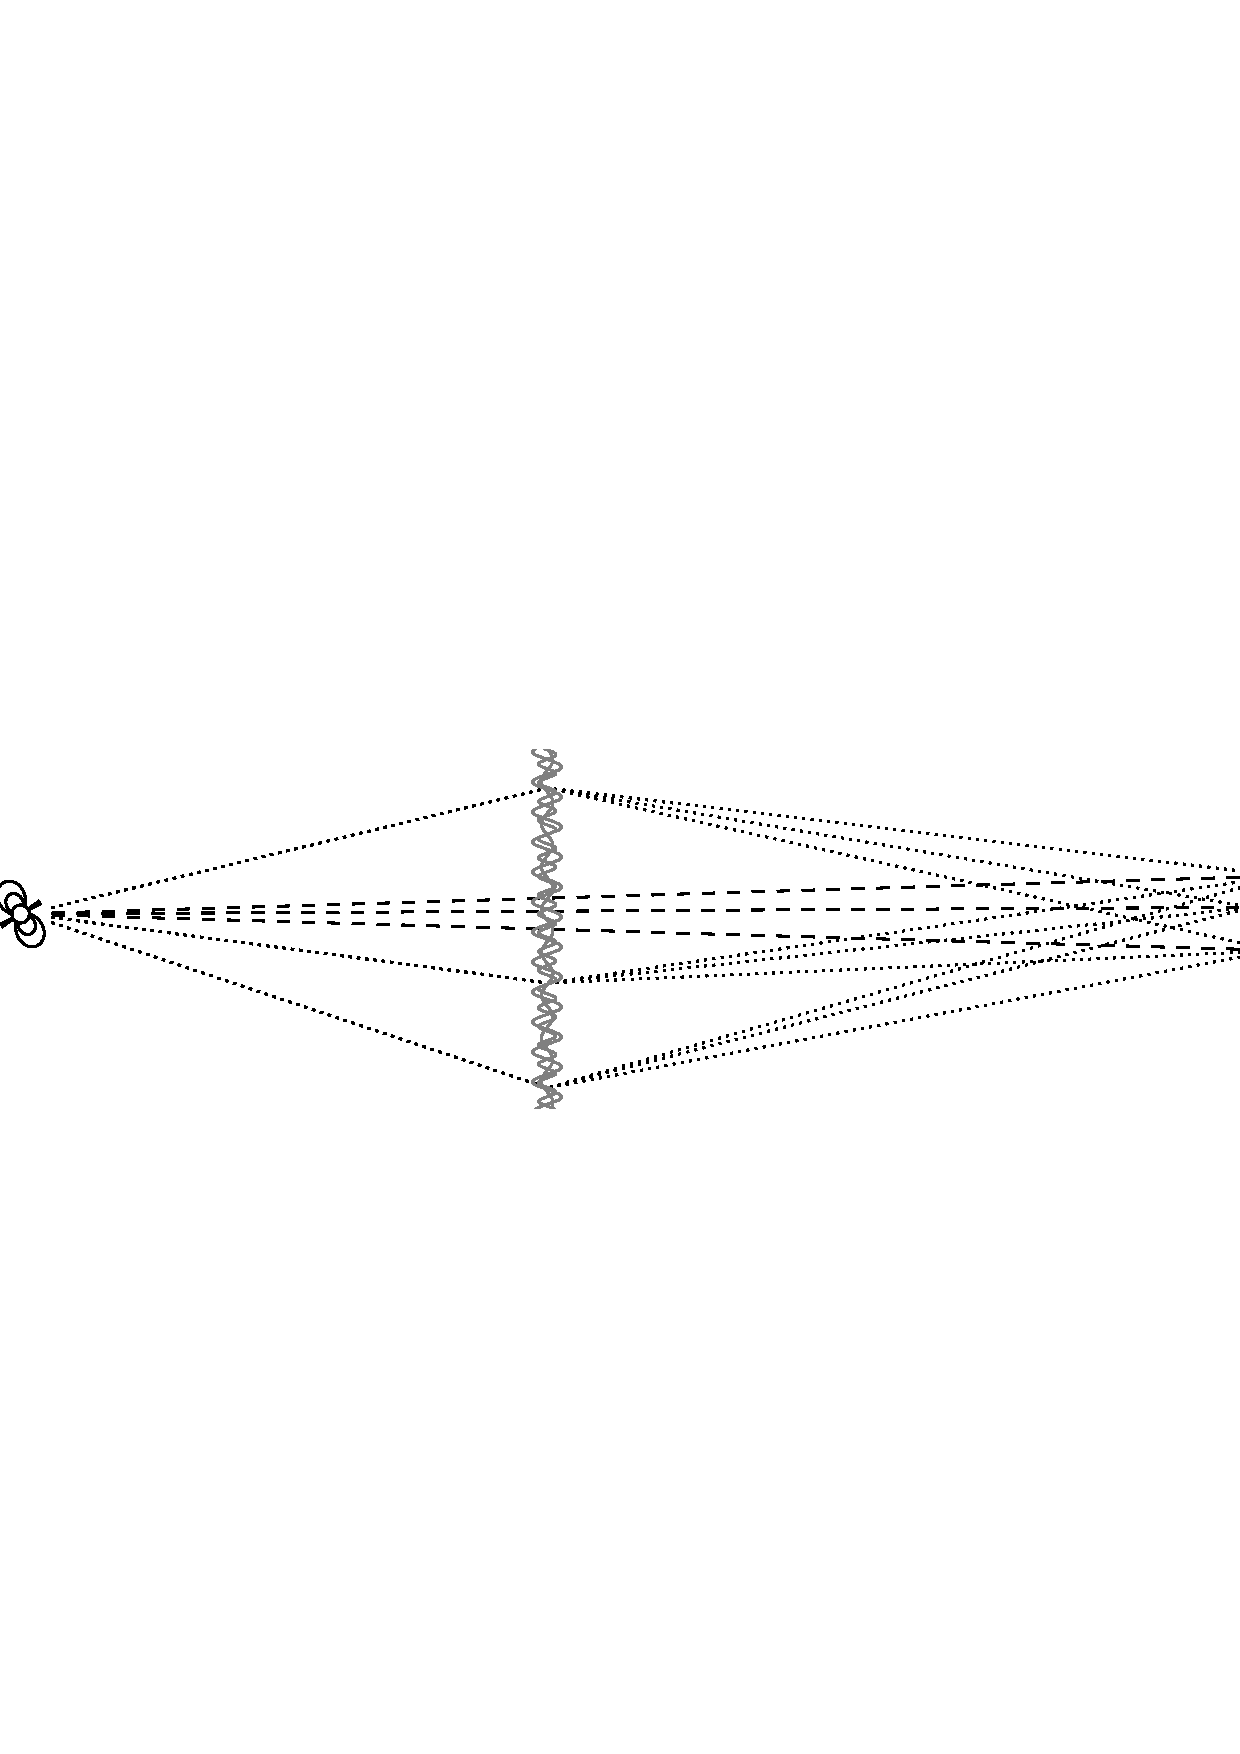
\includegraphics[width=4in]{Figures/scintillometry.pdf}
}


  \frame{
    \frametitle{First Light}
\includegraphics[width=0.8\textwidth]{Figures/liu-lens.png} \tiny
Brisken+2010, Liu+Pen 2016
  }

  \frame{
    \frametitle{Scintillometry}
    \begin{itemize}
    \item map magnetospheres: first fringes on crab with GMRT-MWA,
      DRAO-ARO, EVN, radioastron
    \item preliminary map of magnetosphere: pulse-interpulse widely
      separated, individual GP spatially resolved by nebula during
      strong scattering periods
     \item Magnetosphere mapping for B0834=06, B1957+20 (Main et al 2018)
    \end{itemize}


\vspace{-0.1in}\hspace{1.8in} 
\includegraphics[width=0.4\textwidth]{Figures/allgate.pdf}
\vspace{0.5in}
\tiny Pen+ 2014

.
  }



  \frame{
    \frametitle{Opportunities}
    \begin{itemize}
      \item pathfinding with CHIME: VLBI w/outriggers
      \item initial development at ARO, GB with 10m dishes
      \item slow tree pulsar search
      \item propagation mitigation for pulsar timing: daily CHIME
        monitoring for hundreds of pulsars!
      \item science development well matched to CHORD
    \end{itemize}
  }

  \frame{
    \frametitle{Conclusion}
    \begin{itemize}
      \item pulsars as clocks: PTA precision localization
      \item pulsars as masers: unique probe of the ISM, IGM, BH
      \item coherent emission mechanism, protype for FRBs
      \item unique window for Canadian leadership
    \end{itemize}
  }

\end{document}
